\chapter{Stand der Technik}
\begin{onehalfspace}  
    \label{sec:theorie/standdertechnik}
        In diesem Kapitel wird der Stand der Technik näher beleuchtet. Der Fokus liegt dabei auf den Themen Daten, \ac{KI} und Bias. Zu Beginn wird auf basis der Literatur erläutert, was Daten sind, was Datenqualität bedeutet und worum es sich bei einem Bias handelt. Daraufhin wird näher auf \ac{KI}, das Teilgebiet \ac{ML} und die Ethik in der \ac{KI} eingegangen. Zuletzt werden die Themen in einen gemeinsamen Kontext gebracht und der Einfluss eines Bias auf eine \ac{KI} betrachtet sowie Gegenmaßnahmen untersucht. 
    
    \section{Daten als wertschöpfende Ressource}
    \label{subsec:datenchapter}
    \subsection{Daten}
    \label{subsubsec:daten}
        Dass Daten eine wertvolle Ressource seien, meinte bereits 2006 der britische Mathematiker Clive Humby mit dem berühmten Zitat: \glqq{}Data is the new oil\grqq{}.\cite{Frorbes2021} Hiermit ist gemeint, dass Daten in ihre Rohform nicht sonderlich wertvoll sind, diese jedoch an Wert gewinnen, sobald man beginnt sie zu verarbeiten. Denn lange Zeit waren Daten nur ein Nebenprodukt der Digitalisierung. Daten wurde gesammelt und gespeichert, aber nicht weiter verwendet. Mit dem technologischen Fortschritt im Bereich von Datenanalysen und mit aufkommen der \ac{KI} wurden Daten von Zeit zu Zeit immer wertvoller. So wurden neue Datengetriebene Geschäftsfeld ermöglicht, die einen Mehrwert aus Rohdaten schaffen können. Insbesondere das rasante Aufkommen des Internet of Things hat diese Entwicklung stark vorangetrieben. Seither steigt die Menge der jährlich gesammelten Daten exponentiell an.\cite{Otto2019}
        \\
        \begin{figure}[h]
            \centering
            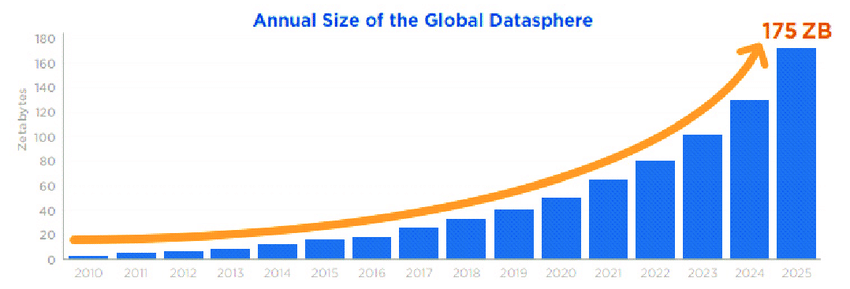
\includegraphics[width = 15.5cm]{Bilder/Annual_Data_Size.png}
            \caption{Weltweit jährlich anfallende Datenmenge \cite{Reinsel2018}}
            \label{fig:DataSize}
        \end{figure}
        \\
        Abbildung \ref{fig:DataSize} stammt aus dem Jahr 2018 und verdeutlicht, dass bereits damals erwartet wurde, dass bis im Jahr 2025 rund 175 Zetabyte Daten jährlich gesammelt werden. Im Vergleich dazu waren es 2018 gerade einmal 33 Zetabyte weltweit.\cite{Reinsel2018}\cite{Taleb2018}
        \\
        Der Begriff Daten selbst wird im ISO2382-1 Standard wie folgt definiert: \glqq{}reinterpretierbare Darstellung von Informationen in einer formalisierten Weise, die für die Kommunikation, Interpretation oder Verarbeitung geeignet ist\grqq{}.\cite{ISO2382} Daraus lässt sich ableite, dass Daten Informationen der Vergangenheit repräsentieren und für zukünftige Verwendung die Informationen aus der Vergangenheit in einer einheitlichen Form repräsentieren. Damit ist jedoch nicht die einheitliche Form der Daten selbst gemeint. 
        \\
        Daten gibt es in unterschiedlichen Formen. Es wird zwischen strukturierten und unstrukturierten Daten unterschieden. Strukturierte Daten sind Datensätze bestehend aus einzelnen Variablen die eindeutige Größen Darstellen. Beispiel hierfür sind Sensordaten oder Unternehmenszahlen aus einem ERP System. Sie werden tabbelarisch gespeichert und können einfach weiter verarbeitet werden. Oftmals sind diese Daten heterogen, was bedeutet, dass sich die Variablen unterscheiden und bspw. Spalte 1 vollkommen andere Daten behinhaltet als Splate 2. Ein Beispiel hierfür wären Sensoren für Luftfeuchtigkeit und Helligkeit in einem Büro. Als unstrukturierte Daten bezeichnet man Daten, die nicht in sinnvolle einheitliche Variablen unterteilt werden können. Zu dieser Art von Daten zählt man Bilder, Videos, Audio und Textdaten. Sie sind meist homogen, denn die Pixel in einem Bild nehmen zwar unterschiedliche RGB Werte an, jedoch repräsentieren sie alle einen Pixel. Dabei ist es egal ob es sich um Pixel 1 oder Pixel 42 handelt.\cite{Horn2022} Bei dieser unvorstellbar großen Datenmenge die jährlich generiert wird, wird davon ausgegangen, dass rund 80\% als unstrukturierte Daten vorliegen.\cite{Otto2019}
        \\
        Häufig wird in dem Zusammenhang mit Daten auch von Big Data gesprochen. Eine einheitliche Definition für den Begriff Big Data existiert jedoch nicht. Denn der Begriff Big Data umfasst die gesamte Wertschöpfungskette. Diese beinhaltet die Datenerzeugung, das Sammel und Speichern der Daten bis hin zur Verarbeitung und Nutzung für Analysen oder Visualisierungen.\cite{Taleb2018}\cite{Faroukhi2020} Es handelt sich dabei um Informationen mit hohem Volumen (high-volume), hoher Geschwindigkeit (high-velocity) und hoher Vielfalt(high-variety). Diese drei charakteristischen Eigenschaften werden in der Literatur auch als die \glqq{}3 V rule\grqq{} bezeichnet und ist in den meisten Definitionen wiederfinden.\cite{Taleb2018}\cite{Yalaoui2021} 
        \begin{figure}[h]
            \centering
            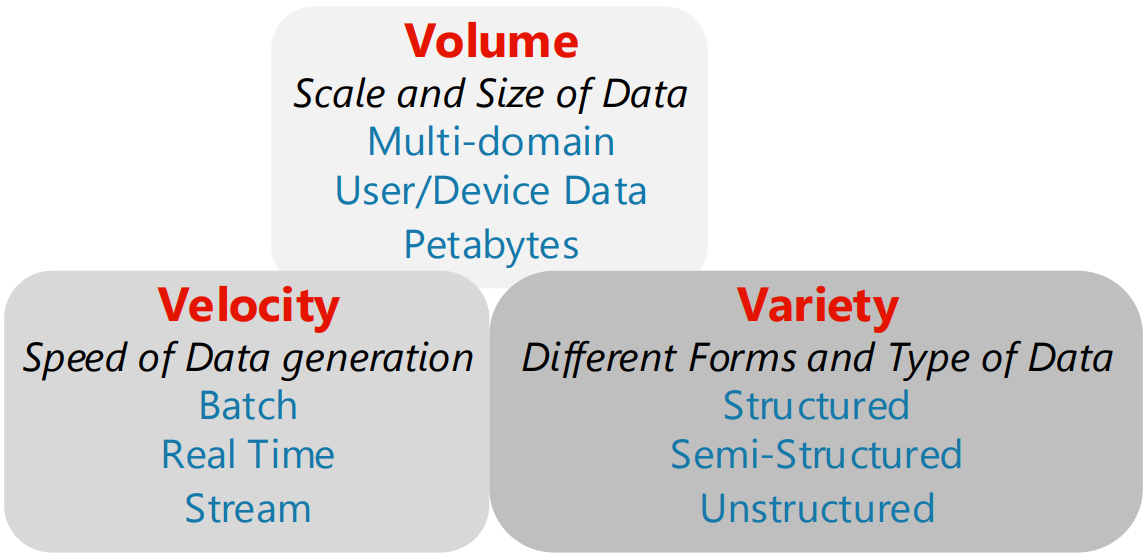
\includegraphics[width = 6.7cm]{Bilder/3VRule.png}
            \caption{Big Data 3 V rule \cite{Taleb2018}}
            \label{fig:3VRule}
        \end{figure}
        \\
        In der Abbildung \ref*{fig:3VRule} werden diese Eigenschaften die Big Data mit sich bringt näher beschrieben. Unter \glqq{}Volume\grqq{} wird die große Menge an Daten, also der damit verbundene benötigte Speicher, und ihre Skalierbarkeit betrachtet. Bei der \glqq{}Velocity\grqq{} liegt der Fokus auf der Geschwindigkeit in der die Daten erzeugt werden. Dies hat wiederrum je nach Geschwindigkeit der Datenerzeugung einfluss auf das Volumen. Abschließend in dem Dreieck gibt es die \glqq{}Variety\grqq{}. Big Data ist von natur aus eine Vielfalt an strukturierten und unstrukturierten Daten. All diese drei Eigenschaften beeinflussen sich gegenseitig und bilden die grundlegenden Eigenschaften von Big Data.
        \\
        In Rohform sind diese Daten, wie eingangs erwähnt, jedoch nicht sonderlich von Wert. Egal ob Big Data oder nicht, einen Mehrwert und Infromationen liefern sie erst, sobald man sie nutzt. Dabei ist es egal ob für Simulationen, Monitoring oder \ac{KI}. In der Vergangenheit sind Daten ein Nebenprodukt der Digitalisierung gewesen. Heute sind sie ein eigenes Geschäftsfeld und \glqq{}Enabler\grqq{} für viele bisher nicht möglich gewesenen Anwendungen.\cite{Otto2019}\cite{Gröger2021}

    \subsection{Datenqualität}
    \label{subsubsec:datenqualität}
        Im Zusammenhang mit Daten fällt immer häufiger auch der Begriff Datenqualität. Hier trifft Quantität auf Qualität. Wie bereits erwähnt, ist die Menge an Daten die bereits zur Verfügung steht, rießig. Quantität ist daher nicht das Problem. Die Qualität der Daten hat hier jedoch sehr großen Einfluss. Nicht selten können Daten nicht verwendet werden, da die Qualität nicht ausreichend ist. Gerade für Analysen, Auswertungen und Vorhersagen, wie sie durch die \ac*{KI} getroffen werden sollen, wird hohe Datenqualität benötigt.\cite{Byabazaire2020}
        \\
        Datenqualität selbst lässt sich auf unterschiedliche Arten und Weisen verstehen.\cite{Yalaoui2021} Eine gängige Definition für Datenqualität in der Literatur ist:\glqq{}fitness for use\grqq{}.\cite{Faroukhi2020} Es bedeutet, dass die Datenqualität von Nutzungskontext und Anwendungsfall abhängt und in erster Linie nicht allgemeine Qualitätsanforderungen erfüllt werden, sondern die für den Use Case benötigten Qualitätsanfoderungen.\cite{Faroukhi2020}\cite{Yalaoui2021}
        \begin{figure}[h]
            \centering
            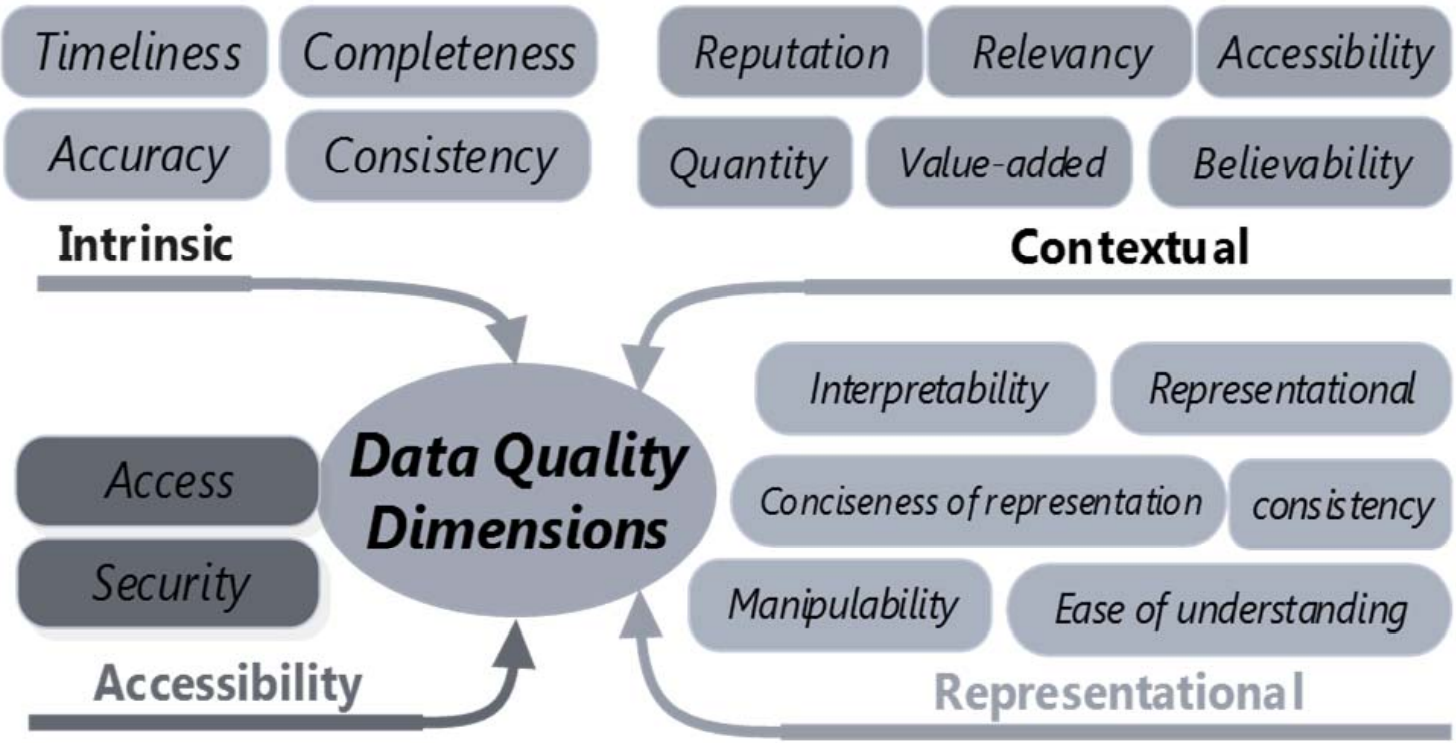
\includegraphics[width = 9cm]{Bilder/Data_quality_dimensions.png}
            \caption{Data Quality Dimensions \cite{Taleb2018}}
            \label{fig:DataQualityDimensions}
        \end{figure}
        \\
        Für die Validierung der Datenqualität gibt es die sogenannten Data Quality Dimensions. In Abbildung \ref{fig:DataQualityDimensions} sind die vier unterschiedlichen Dimensionen: Intrinsic (\ac{dt}.: Intrinsisch), Contextual (\ac{dt}.: Kontextbezogen), Accessibility (\ac{dt}.: Zugänglichkeit ) und Representational (\ac{dt}.: Repräsentativ) dargstellt. Jede Dimension besitzt eigene Merkmale an denen die Datenqualität gemessen werden kann. Näher erläutert werden die Dimensionen in der Tabelle \ref*{table:0}.
        \\
        \begin{table}[h]
            \centering
            \begin{adjustbox}{width=\textwidth}
            \resizebox{\textwidth}{!}{\begin{tabular}{|l|l|}
            \hline
            Intrinsic        & \begin{tabular}[c]{@{}l@{}}
                                    Zur intrinsischen Datenqualität gehören, wie in Abbildung \ref*{fig:DataQualityDimensions} zu sehen,\\
                                    die Merkmale: Zeitlos, Vollständigkeit, Genauigkeit, Konsistenz. Die \\
                                    intrinsische Dimension bildet die Qualitätsmerkmale der Daten selbst ab. \\
                                    und gibt Aufschluss über Objektivität und Glaubwürdigkeit der Daten.\cite{Yalaoui2021}
                                \end{tabular}  \\ \hline
            Contextual      &   \begin{tabular}[c]{@{}l@{}}
                                    Bei der kontextbezogenen Datenqualität wird betrachtet in welchem Ausmaß \\
                                    die Daten für den Nutzenden einsetzbar sind. Darin werden Eigenschaften wie:\\
                                    Datenmenge (Quantität), Zugänglichkeit, Aktualität und Mehrwert \\
                                    der Daten betrachtet um die Nutzbarkeit zu messen.\cite{Otto2019}
                                \end{tabular}  \\ \hline
            Representational &  \begin{tabular}[c]{@{}l@{}}
                                    Repräsentativ bedeutet im Kontext der Datenqualität, dass die Daten \\
                                    Interpretierbarkeit und dabei primär einfach zu Verstehen sind, \\
                                    Konsistaent sind und  Manipulierbarkeit, also Veränderbar sind.\cite{Byabazaire2020}

                                \end{tabular}  \\ \hline
            Accessibility    &  \begin{tabular}[c]{@{}l@{}}
                                    Die vierte Dimension, die Zugänglichkeit, bezieht sich Insbesondere \\
                                    auf das Speichersystem der Daten. Diese Dimension wird an der möglichst\\
                                    einfachen Zugänglichkeit und der entgegenstehenden Sicherheit der \\
                                    Daten gemessen.\cite{Byabazaire2020}
                                \end{tabular}  \\ \hline           
            \end{tabular}}
            \end{adjustbox}
            \caption{Data Quality Dimensions Merkmale}
            \label{table:0}
        \end{table}
        \\
        Datenqualität lässt sich in unterschiedlichsten Dimensionen und anhand unterschiedlicher Qualitätsmerkmale messen. Die in Abbildung \ref*{fig:DataQualityDimensions} dargestellten und in Tabelle \ref*{table:0} erläuterten Dimensionen sind dabei nur eine der gängigen Modelle aus der Literatur. 
        \\
        Trotz des Bewusstseins für Datenqualität, besteht rund 80 Prozent der Arbeit eines Data Scientist daraus, Daten aufgrund von Qualitätsanfoderungen vorzuverarbeiten.\cite{Horn2022} Angefangen beim einfachen Umwandeln bis hin zu komplexeren Bereinigungen und Encodierungen der Daten. Daten werden in den meisten Fällen nicht die gewünschten Qualitätsanforderungen erfüllen können. Datenqualität ist keine verallgemeinerbare Formel, sondern immer abhängig vom Anwendungsfall und dem Kontext in dem die Daten genutzt werden sollen.
        \\
        Dass Datenqualität eine wichtige Rolle spielt, unabhängig von dem Verwendungszweck, ist keine Frage. In der Wissenschaft sowie Wirtschaft wird sich immer intensiver mit der Thematik der Datenqualität auseinandergesetzte, da heutzutage die Quantität kam noch ein Problem darstellt, sondern viel mehr die Qualität der Daten.\cite{Lis2019} Denn Quantität ist nicht gleich Qualität!

%#########################################

    \newpage
    \section{Künstliche Intelligenz}
    \label{subsec:KIandML}
    \subsection{Künstliche Intelligenz Allgemein}
    \label{subsubsec:KIAllgemein}
        \ac{KI} als Begriff wird vielseitig und unterschiedlich Verwendet. Die Vision von \ac{KI} ist es, die intellektuellen und menschlichen Fähigkeiten als ein KI-System nachzubilden.\cite{Lis2019} Letztendlich beschreibt \ac{KI} ein Forschungsbreich aus der Informatik, der aus einer Vielzahl aus Technologien besteht.\cite{HEGKI2019Definition} 
        \begin{figure}[h]
            \centering
            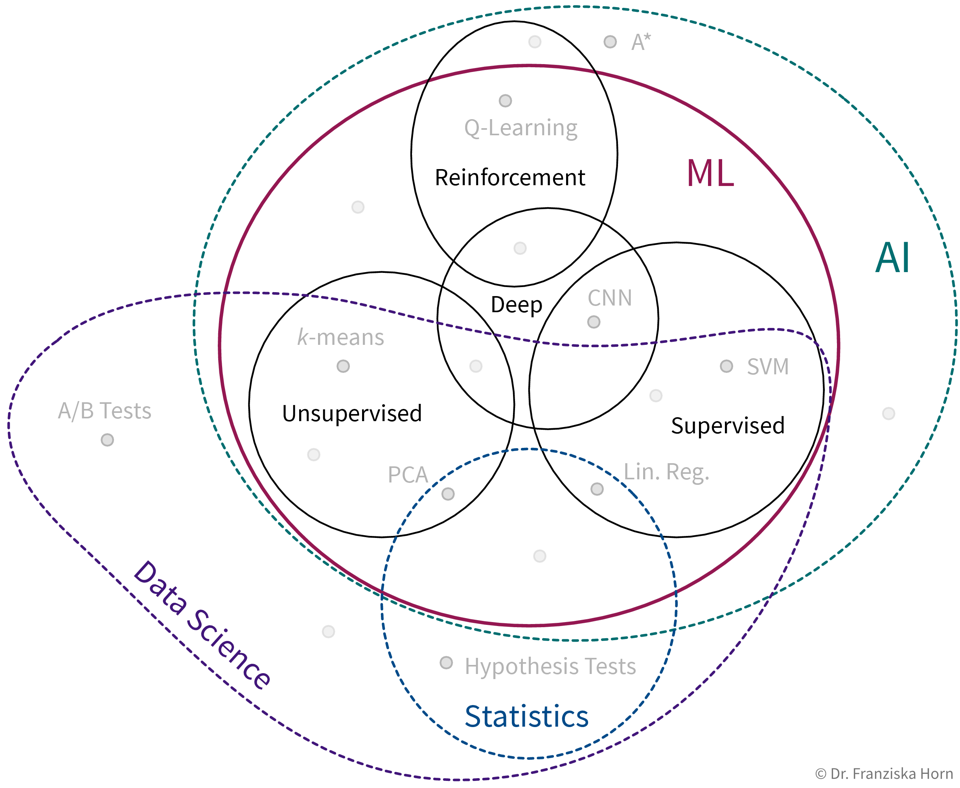
\includegraphics[width = \textwidth]{Bilder/ml_toolset.png}
            \caption{Exemplarisch dargestellte Disziplinen von \ac{KI}\cite{Horn2022}}
            \label{fig:ml_toolset}
        \end{figure}
        \\
        Die Abbildung \ref*{fig:ml_toolset} ziegt exemplarisch, welche Position \ac*{KI} in der Infromatik einnimmt. Zur \ac{KI} gehören bekannte Teilgebiet wie das \ac*{ML}, Optimierungsalgorithmen, aber auch  in der Robotik kommt \ac{KI} zum Einsatz. Selbst wird die Disziplin aber auch von anderen übergeordneten Disziplinen genutzt.\cite{HEGKI2019Definition} Ein Beispiel hierfür ist Data Science. Die Abbildung \ref*{fig:ml_toolset} veranschaulticht, dass einige Aspekte aus der \ac{KI} im Bereich Data Science augegriffen werden, jedoch deutlich mehr als nur \ac{KI} hinter Data Science steckt.
        \\
        In der Literatur wurde in der Vergangenheit oft zwischen \glqq{}schwacher\grqq{} und \glqq{}starker\grqq{} \ac{KI} unterschieden. Eine schwache \ac{KI} ist dabei für ein spezifisches Anwendungsproblem konzipiert. Der \ac{KI} wird eine Aufgabe gegeben und diese versucht mittels Algorithmen und mathematischen Funktionen die Aufgabe zu lösen. Diese Art der \ac{KI} versucht Aufgaben zu lösen und Ergebnisse zu liefern, wie sie durch menschliche Intelligenz entstehen können.\cite{Lis2019} Ein Beispiel hierfür ist die Bilderkennung, bei der Entschieden wird, ob auf dem Bild eine Erdbeere zu sehen ist, oder nicht.
        \\
        Als starke \ac{KI} wird ein System verstanden, welches in der Lage ist ein breites Spektrum an Aufgaben zu erledigen.\cite{Datenkommission2019} Sie verfügt über weitere Methoden zur Datenverarbeitung. In dieser Form der \ac{KI} wird mehr versucht die menschlichen Fähigkeiten und Intelligenz abzubilden. Es wird nicht nach eine spezifischen Vorgehensweise vorgegangen, sondern Aufgaben werden mit individuellen Lösungenswegen erledigt.\cite{Lis2019}
        \\
        Mit dem Begriff \ac{KI} wird demzufolge nur ein grundlegendes Prinzip von \ac*{KI}-Systemen definiert. Die Aufgabe dieser \ac*{KI}-Systeme ist es, Daten jeglicher Form zu interpretieren, Schlussfolgerungen daraus zu ziehen und eine Aussage über das zu erreichende Ziel zu liefern. Unabhängig davon, ob es sich um einen optimalen Lösungsweg, eine Vorhersage oder eine Schlussfolgerung handelt. \cite{HEGKI2019Definition}    
    
    \subsection{Teilgebiet maschinelles Lernen}
    \label{subsubsec:teilgebietML}
        Maschinelles Lernen ist das Teilgebiet der \ac{KI}, welches häufig als \ac*{KI} bezeichnet wird. Unter \ac{ML} wird verstanden, dass ein \ac*{ML} Modell von Lernalgorithmen entwickelt wird, welches in der Lage ist, das Wissen aus Erfahrungen anzuwenden. Dabei soll dem Modell ein unbekannter Input geliefert, dieses verarbeitet die Eingabewerte mit dem Wissen welches es besitzt und liefert ein Ergebnis als Output zurück. Der Output ist dabei abhängig von der zu lösenden Aufgabe. Klassische Anwendungsfälle von \ac*{ML} sind daher Vorhersagen, Schlussfolgerungen, Optimierungen, Entscheidungen, Sprach- und Bilderkennung \ac*{bzw} Verarbeitung und weitere ähnliche Aufgaben.\cite{HEGKI2019}
        \\
        Um das Teilgebiet \ac{ML} genauer zu betrachten, unterscheidet man in der Literatur zwischen \glqq{}superviced learning\grqq{}(\ac*{dt}.: überwachtes Lernen), \glqq{}unsuperviced learning\grqq{}(\ac*{dt}.: unüberwachtes Lernen) und dem \glqq{}reinforcement learning\grqq{}(\ac*{dt}.: bestärktes Lernen).\cite{Datenkommission2019} Diese Unterscheidung wird anhand der Art des Lernens getroffen.\cite{Horn2022} In Abbildung \ref*{fig:ml_algorithms}, werden diese unterschiedlichen Änsätze des Lernens vereinfacht dargestellt. 
        \begin{figure}[h]
            \centering
            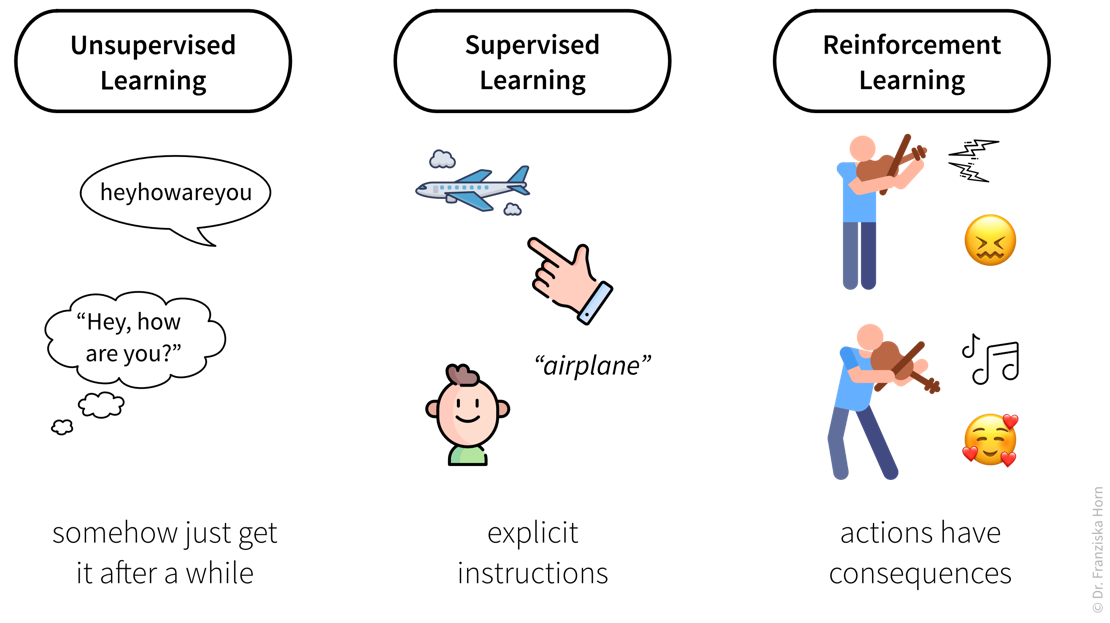
\includegraphics[width = 14cm]{Bilder/ml_algorithms.png}
            \caption{Arten des maschinellen Lernen\cite{Horn2022}}
            \label{fig:ml_algorithms}
        \end{figure}
        \\
        Das \glqq{}unsuperviced learning\grqq{}(\ac*{dt}.: unüberwachtes Lernen), in der Abbildung \ref*{fig:ml_algorithms} links dargestellt, basiert auf dem Prinzip, dass dem Modell ein Input ohne zusätzliche Informationen gegeben wird und das Modell selbstständig Zusammenhänge erlernt. Lediglich die zu suchende Struktur ist dem Modell zu liefer, damit ist gemeint, ob nach bspw. Ausreißern gesucht werden soll. In der Abbildung  \ref*{fig:ml_algorithms}, wird dies an dem Beispiel eines Texts veranschaulicht. Dem Modell wird lediglich die Buchstabenkette gegeben und dieses erkennt darin die einzelnen Wörter und, dass es sich um eine Frage handelt. Ein häufiger Anwendungsfall für das unüberwachte Lernen ist das Clustering, da das Modell in den Daten Zusammenhänge erkennt, die ein Mensch nicht direkt sieht.\cite{Datenkommission2019}\cite{Döbel2018} \\
        Bei dem \glqq{}superviced learning\grqq{}(\ac*{dt}.: überwachtes Lernen), wird ein sehr Menschen ähnliches Lernverfahren genutzt. Vereinfacht gesagt wird bei dieser Art des Lernens etwas vorgemacht/erklärt und das Modell merkt sich diesen Zusammenhang. Auf diese Art und weiße erlernt das Modell Strukturen und kan dies auf ihm unbekannte Daten anwenden. Das Beispiel aus Abbildung \ref*{fig:ml_algorithms} veranschaulicht diesen Lernverfahren. Hier wird auf ein Flugzeug gezeigt und dem Kinde gesagt, dass es sich um ein Flugzeug handelt. Das Kind merkt sich diesen Zusammenhang und ist beim nächsten mal selbst in der Lage das Flugzeug zu erkennen und es so zu benennen. Die gängigen Anwendungsfelder des überwachten Lernen sind Vorhersagen und Entscheidugen.\cite{Döbel2018} \\
        Die dritte und bisher am wenigsten verbreitete Art des Lernens ist das \glqq{}reinforcement learning\grqq{}(\ac*{dt}.: bestärktes Lernen). Es handelt sich dabei um Feedback basiertes Lernen. Es bedeutet, dass das Modell eine Auswahl an Handlungen hat, aus denen das Modell frei entscheiden darf, welche ausgeführt wird. Die Entscheidungen werden erst im Nachgang bewertet und in Form einer meist numerischen Bewertung an das Modell zurück gegeben. So lernt das Modell, wenn es etwas gut gemacht hat oder auch falsche Handlungen ausgeführt hat. In Abbildung \ref*{fig:ml_algorithms}, wird dies anhand einer musizierenden Person dargestellt. Die Person spielt etwas auf ihrem Instument und bekommt nach dem Spielen eines Tons das Feedback der Zuhörenden ob es sich gut anhört oder nicht. So lernt die Person wann sich etwas gut anhört und verbessert durch das Feedback ihr können. Häufig findet das bestärkende Lernen deshalb Einsatz in der Robotik, in der ein Roboter anhand von Feedback Bewegungsabläufe erlernt. Bekannt ist hier eine Roboter, der eine menschliche Hand nachbildet und erlernt einhändig einen Rubik’s Cube zu lösen.\cite{Horn2022}\cite{Döbel2018}\cite{Rubik2019}
        \\
        Im Rahmen dieser Arbeit wird der Fokus speziell auf das superviced Learning gelegt. Denn überwahtes Lernen komm meist dann zum Einsatz, wenn Vorhersagen oder Entscheidungen getroffen werden. Dieser Aspekt wird im Verlauf der Arbeit immer wieder eine Rolle spielen. Einzigartig am überwachten Lernen ist, wie bereits erwähnt, dass zum Lernen von Zusammenhängen immer ein \glqq{}Lehrer\grqq{} benötigt wird. Im Falle eines \ac{ML} Modells handelt es sich dabei nicht um eine Lehrer, sondern um Daten, genauer gesagt Trainingsdaten.
        Das Prinzip nach dem das überwachte Lernen funktioniert, ist in Abbildung \ref*{fig:learningProcess} exemplarisch anhand eines Beispiels dargestellt.
        \begin{figure}[h]
            \centering
            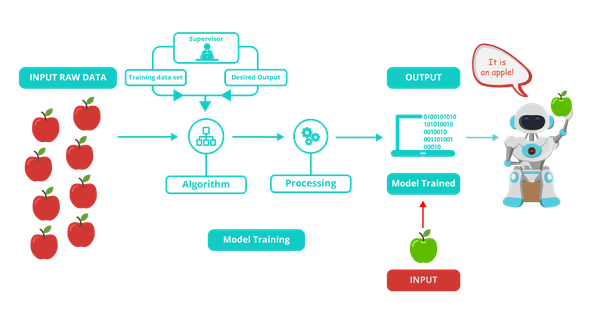
\includegraphics[width = 14cm]{Bilder/superviced_learning.png}
            \caption{Der Prozess von überwachtem Lernen \cite{Kharwal2020}}
            \label{fig:learningProcess}
        \end{figure}
 %       ZU ÜBERARBEITEN
        \\
        Zu Beginn wird das zu lösende Problem definiert, dabei geht es darum die Lernaufgabe des Modells festzulegen. Beim überwachten Lernen wird zwischen Regressionen und Klassifikation unterschieden. Regressionen kommen meist bei Schlussfolgerungen oder Vorhersagen zum Einsatz und Klassifikationen bei Entscheidungen. 
        Anhand des Problems wird dann ein Alogirthmus als Grundlage für das Modell ausgewählt. Um den Modell nun Wissen beizubringen werden sogenannte Trainingsdaten verwendet. Dabei handelt es sich um Daten in dem Format, wie sie auch später im Betrieb als Eingaben X geliefert werden. Diese werden jedoch davor mit Labels versehen. Diese Labels werden durch Experten für die Trainingsdaten erstellt. Im nächsten Schritt wird dann das Modell auf Basis der Trainingsdaten trainiert. Diese Phase ist die entscheidende Lernphase des Modells. Im prinzip ist das Modell nach dem training bereit für den Einsatz. Meist wird jedoch noch mit einem, dem Modell bisher unbekannten und nicht gelabeldten, Datensatz überprüft ob das Modell richitg funktioniert und die Qualität anhand unterschiedlicher Metirken, wie der Genauigkeit bewertet. Danach ist das Modell einatzbereit und kann mit Eingaben X gespeist werden und schließt dann auf Basis des erlernten Wissens auf eine Ausgabe Y. \cite{Horn2022}\cite{Döbel2018}
        Auf diese Art und weiße werden beim überwachten Lernen die input Output Probleme gelöst. \cite{Ng2018}
        \\
        Es gibt aber auch einige negative Eigenschaften die bei \ac{ML} Modelle zu berücksichtigen sind und zu möglichen Problemen führen können. Die meisten dieser Risiken lassen sich jedoch inzwischen durch Gegenmaßnahmen verhinder. Zu den Häufigsten Problemen gehören zu geringe Datenmengen, die Passgenauigkeit, Scheinkorrelationen und Verzerrungen. 
        \begin{enumerate}
            \item Die Datenmenge ist ein entscheidender Faktor im überwachten Lernen. Viele Modelle scheitern daran, dass sie auf Basis von zu wenigen Trainingsdaten trainiert wurden und so nicht in der Lage sind treffende Schlüsse zu ziehen. \cite{Datenkommission2019}\cite{Ng2018}
            \begin{figure}[h]
                \centering
                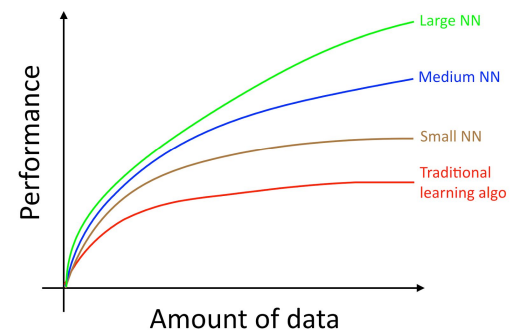
\includegraphics[width = 8cm]{Bilder/Datenmenge.png}
                \caption{Veränderung der Performance durch die Datenmengen \cite{Ng2018}}
                \label{fig:Datavolume}
            \end{figure} 
            In Abbildung \ref*{fig:Datavolume} ist der Zusammenhang zwischen der Datenmenge und der Performance des Modells dargestellt. Hier wird zwar des spezielle Fall von unterschiedlich großen Neuronalen Netzen betrachtet, jedoch lässt sich dies auch auf allgemein \ac*{ML} übertragen. Der Verlauf ähnelt dem eines beschränkten Wachstums. Das bedeutet für das Modell, dass es zu Beginn mit einer ausreichenden Datenmenge möglich ist eine gute Performance zu erziehlen, jedoch um später wenige Prozente an Verbesserung zu erziehlen werden sehr große Datenmengen benötigt.\cite{Ng2018} In einigen Szenarien existieren aber von Beginn an zu wenig Daten für eine gute Performance. Als Gegenmaßnahme können lediglich mehr Daten generiert und gesammelt werden.
            \item Bei der Passgenauigkeit wird ein Problem bei dem Modell selbst adressiert, nämlich das overfitting (\ac*{dt}.: \glqq{}überangepasst\grqq{}) und underfitting (\ac*{dt}.: \glqq{}unterangepasst\grqq{}). Vereinfacht gesagt, wird beim overfitting der Trainingsdatensatz durch das Modell zu genau repräsentiert. Erkennbar wird overfitting, wenn man die Performance von dem Modell bei einem Trainings- und eine Testdatensatz betrachtet. Ist die Performance bei den Trainingsdaten akzeptabel und bei den Testdaten deutlich schlechter, ist es nahezu sicher, dass das Modell zu sehr auf die Trainingsdaten angepasst ist.
            Beim underfitting hingegen, ist die Performance bei beiden Datensätzen nicht akzeptabel. Das liegt daran, dass beim underfitting zu wenig Zusammenhänge erlernt wurden und so keine realistischen Ergebnisse reproduziert werden können.
            \begin{figure}[h]
                \centering
                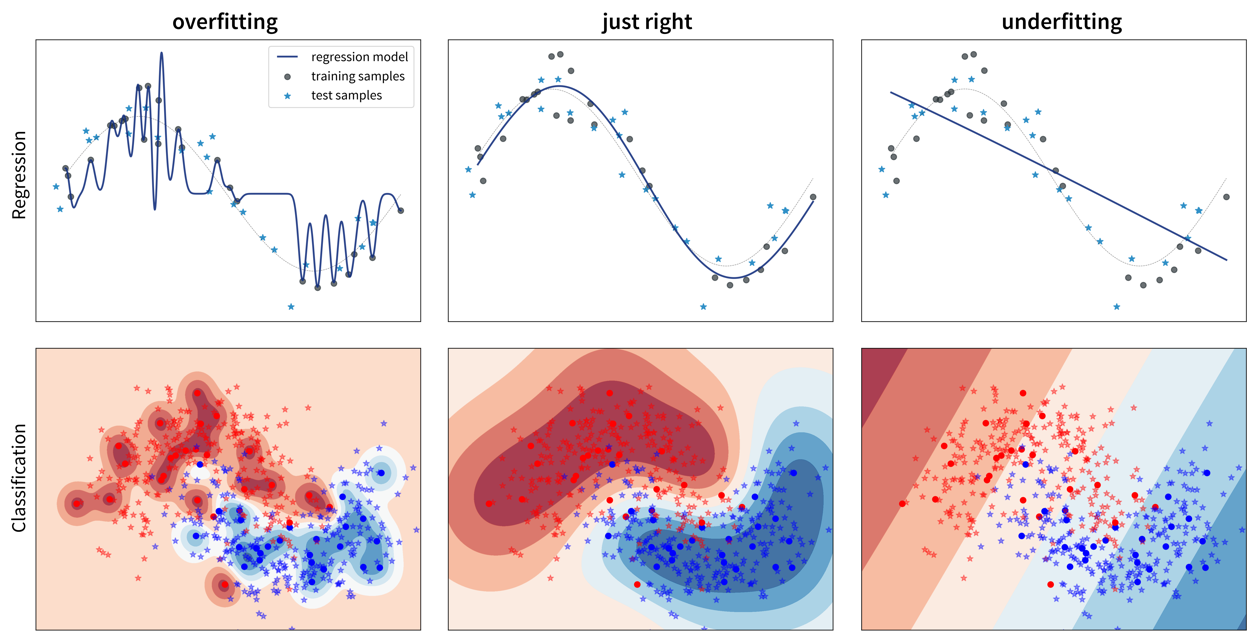
\includegraphics[width = 12cm]{Bilder/overunderfitting.png}
                \caption{Overfitting und Underfitting \cite{Horn2022}}
                \label{fig:Fitting}
            \end{figure}
            Diese Problematik wird in Abbildung \ref*{fig:Fitting} veranschaulicht. Auf der linken Seite ist ein überangepasstes Modell, welches den Trainingsdatensatz \glqq{}auswenig gelernt\grqq{} hat und nicht auf neue Datenpunkte verallgemeinern kann. Rechts ist das unterangepasste Modell zu sehen, welches den Zusammenhang von Input und Output nicht abbilden kann und zu ungenau ist, da es \glqq{}zu wenig gelernt\grqq{} hat.\cite{Horn2022}
            \item Nicht nur overfitting und underfitting sorgen in Modellen für ungenauigkeiten auch Scheinkorrelationen sind häufig eine Fehlerursache. Bei Scheinkorrelationen, werden von dem Modell Zusammenhänge erlernt, die keinerlei Zusammenhang mit der tatsächlichen Entscheidung haben.
            \begin{figure}[h]
                \centering
                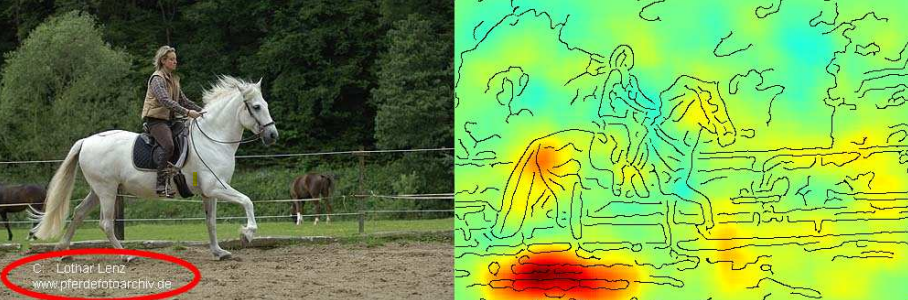
\includegraphics[width = 12cm]{Bilder/Scheinkorrelation.png}
                \caption{Scheinkorrelationen in der Bilderkennung \cite{Lapuschkin2016}}
                \label{fig:Scheinkorrelation}
            \end{figure} \\
            Ein Beispiel dafür ist in Abbildung \ref*{fig:Scheinkorrelation} zu sehen. In der ein Pferdebild nicht anhand der Kontur des Pferdes, sondern anhand des Wasserzeichens in dem Bild erkannt wurde. Grund dafür war, dass einige der Trainingsdaten dieses Wasserzeichen beinhaltet haben und das Modell daraus eine Scheinkorrelation erlernt hat. \cite{Horn2022}\cite{Lapuschkin2016}\cite{Cremers2019}
            \item Ein letztes und schwerwiegendes Problem ist die Verzerrung von Trainingsdaten, auch Bias genannt. Dieser Aspekt wird später in Kapitel \ref*{subsubsec:Bias} genauer betrachtet. Allgemein kann man sagen, existieren Verzerrungen in Trainingsdaten, so wird das Modell diese Verzerrungen reproduzieren.\cite{Cremers2019}
        \end{enumerate}
        Zusammenfassend wird bei \ac*{ML}, speziell beim überwachten Lernen auf Basis von Daten, Trainingsdaten genannt, Wissen aus der Vergangenheit erlernt. Dazu werden Zusammenhänge in den Daten genutzt und die dazugehörigen Bewertungen in Form von Labels. So entsteht eine äbhängigkeit des Modells von den Trainingsdaten. Im Falle von zu wenig Trainingsdaten, wird das Modell die Realität unterrepräsentieren und daher nicht einsetzbar. Die Daten selbst können aber ebenfalls zu Scheinkorrelationen und Verzerrungen führen die das Ergebnis des Modells mitunter stark beeinflussen. \cite{Cremers2019}
 
    \newpage
    \subsection{Ethik in der künstlichen Intelligenz}
    \label{subsubsec:ethikinderKI}
        Ein Aspekt der bisher nicht beleutet wurde ist die Ethik. Die Ethik spielt in der \ac{KI} eine immer größer werdende Rolle. In einer Gesellschaft die für Inklusion steht, werden häufig Entscheidungen hinterfragt und kritisiert. Dies gilt insbesondere für Entscheidungen und Vorhersagen, die durch \ac{KI} getroffen werden und so ohne direkten menschlichen Einfluss getroffen werden.
        \begin{figure}[h]
            \centering
            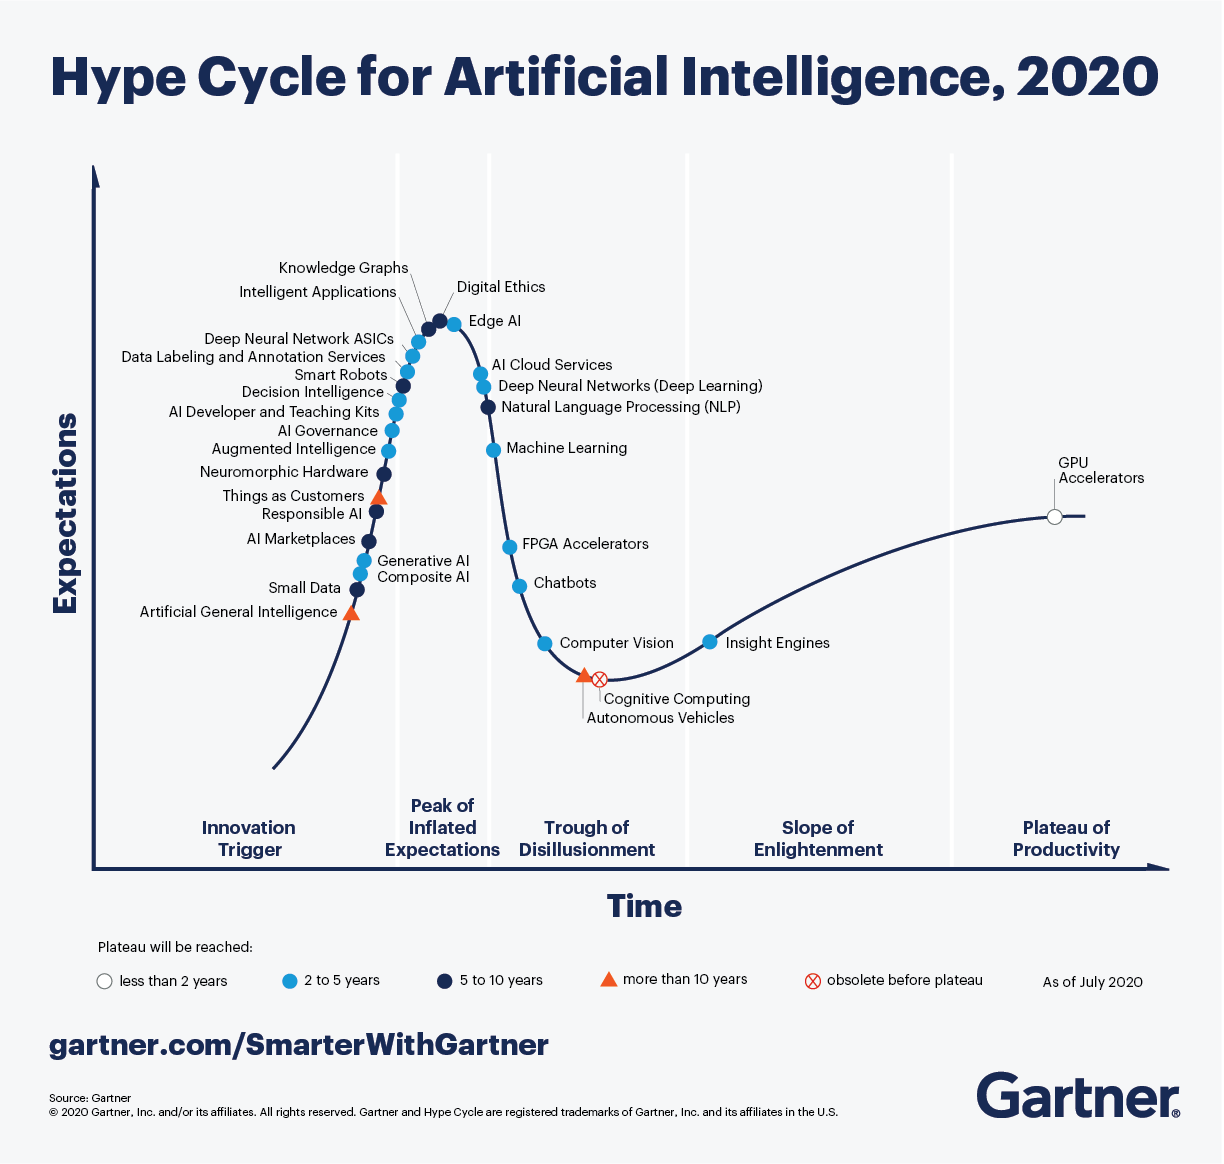
\includegraphics[width = 14cm]{Bilder/Gartner_hypeCycle.png}
            \caption{Gartner Hype Cycle für \ac*{KI} \cite{Goasduff2020}}
            \label{fig:HypeCycle}
        \end{figure}
        \\
        Im Gartner Hype Cycle für \ac*{KI} aus dem Jahr 2020, dargestellt in Abbildung \ref*{fig:HypeCycle}, wurde das Thema Digitale Ethik auf dem Höhepunkt der Kurve platziert. Der Forschungsbreich rund um die digitale Ethik befindet sich jedoch erst im Anfangsstadium. Trotzdem sind die Erwartungen bereits sehr hoch, denn auch der gesellschaftliche Druck steigt an. Ursache dafür ist unter anderem der Skandal um den Chatbot Tay von Microsoft der innerhalb von nur einem einzigen Tag rassistische \"Außerungen von den Nutzern lernte und daraufhin offline genommen werden musste.\cite{Cremers2019}
        Um einen einheitlichen Rahmen für die Ethik in der \ac*{KI} zu schaffen wurde 2018 von der EU eine Kommision von hochrangigen \ac*{KI} Experten (kurz. HEG KI) gegründer, aber auch Forschungsinstitute setzten sich vermehrt mit der Thematik auseinandern. 2021 waren es allein in Deutschland über 40 Projekte.\cite{Beckert2021}
        \\
        Grundlegend ist die Aufgabe der Ethik in der \ac*{KI}, dass ein Rahmen geschaffen wird, in dem eine \ac*{KI} agiert und dabei keine ethischen Grundprinzipien verletzt.\cite{Cremers2019} Ethik ist jedoch nicht einfach in Form von Code programmierbar und kann daher auch nicht von Grund auf in eine \ac*{KI} integriert werden. In den meisten Fällen ist Ethik und ethische Entscheidungen stark von dem Rahmen und Kontext abhängig. Ziel der Ethik ist es sich so zu verhalten und zu handeln, dass  keine beteilite Person in ihren Rechten bechnitten wird oder einen Schaden erleidet.\cite{Heesen2020}
        Dabei bezieht sich die Ethik für die Vorgabe von Leitlinien meist auf die Grundrechte die in Deutschland durch das Grundgesetz definiert werden. In Zeiten der Digitalisierung reichen diese ethischen Grundsätze jedoch oft nicht aus. Mit immer schneller aufkommenden neun Technologien kommen auch neue Probleme und nicht selten auch ethische Probleme auf. Da die Ethik aber auf historischen Erfahrungen basiert, fehlen diese, um einen klaren Weg vorzugeben. So kommt es, dass die Ethik mehr und mehr eine zentrale Rolle in der Gesellschaft gewinnt, wenn es um den Umgang mit neuen digitalen Technologien geht.\cite{Cremers2019} \\
        Die \ac*{KI} hat die Frage nach Ethik dabei insbesondere damit geprägt, dass Entscheidungen von einem maschinellen Modell getroffen werden, welche in der Vergangenheit oft nicht transparent und nachvollziehbar waren. Für Viele fehlt daher das Vertrauen in eine Entscheidung, die durch einen Computer getroffen wurde. Um diese Bedenken zu minimieren und ein Vertrauen zu schaffen benötigt man Leitlinien für Ethik in der \ac*{KI}.\cite{Heesen2020}
        \\
        Die Ethik wird dabei meist mit dem Konzept von vertrauenswürdiger \ac*{KI} in Verbindung gebracht. In diesem Konzept werden die folgenden drei Anforderungen an eine \ac*{KI} gestellt:
        \begin{enumerate}
            \item \textbf{Rechtmäßigkeit:} \\ Eine \ac*{KI} soll das geltenden Recht und die gesetzlichen Bestimmungen einhalten.
            \item \textbf{Ethik:} \\ Eine \ac*{KI} soll ethische Grundsätze und Werte einhalten.
            \item \textbf{Robustheit:} \\ Eine \ac*{KI} soll technisch Robust gegen Manipulation gestaltet sein.
        \end{enumerate}
        Erfüllt eine \ac*{KI} alle drei Anforderungen gilt sie als eine vertrauenswürdige \ac*{KI}. Ziel des Konzepts ist es, die Vorteile von \ac*{KI} zu maximieren aber gleichzeitig die Risiken, egal ob rechtliche oder ethische, möglichst gering zu halten.\cite{HEGKI2019} Dafür muss eine Grundlage auf Basis der drei Kategorien Recht, Ethik und Technologie geschaffen werden, die nur im zusammenspiel zu einer umsetzbaren vertrauenswürdigen \ac*{KI} führen.
        \\
        Wenn man sich nun mit dem Konzept einer vertrauenswürdigen \ac*{KI} genauer beschäftigt, müssen Fragestellungen, wie sie in Abbildung \ref*{fig:EthikAnforderungen} zu sehen sind, gestellt werden. 
        \\
        \begin{figure}[h]
            \centering
            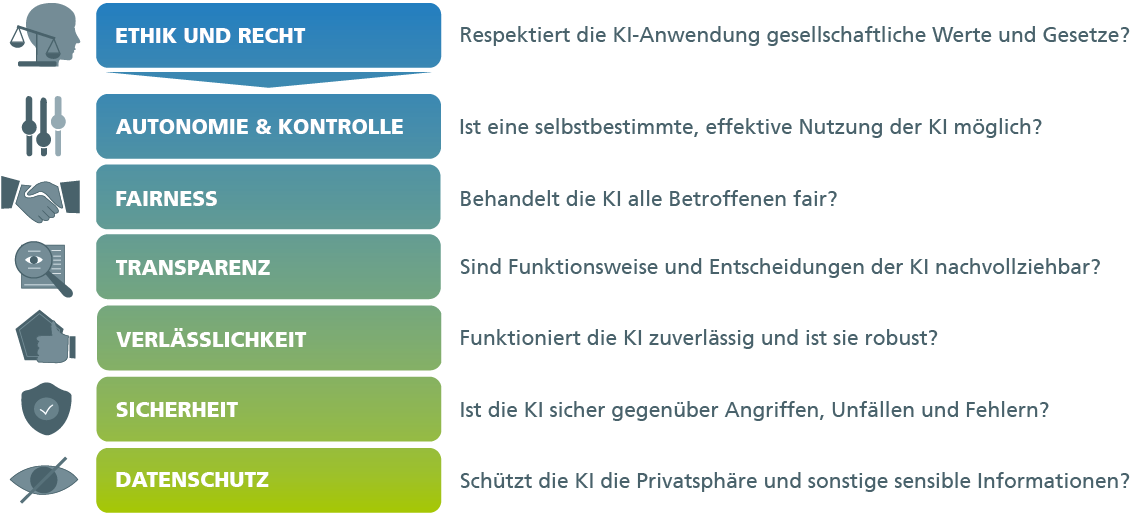
\includegraphics[width = 14cm]{Bilder/Grafik-KI_Whitepaper_final_WEB_2.png}
            \caption{Ethische und rechtliche Grundlagen für eine \ac*{KI} \cite{Cremers2019}}
            \label{fig:EthikAnforderungen}
        \end{figure}
        \\
        Die Abbildung \ref*{fig:EthikAnforderungen} stellt eine Auswahl konkreter Aspekte, der oben beschreibenen Grundsätze, dar. Es sind die einzelnen Aspekte die für eine vertrauenswürdige \ac*{KI} notwendig sind. Begonnen bei ethischen Grundsätzen wie der Autonomie und Fairness bis hin zu klar rechtlich einordbaren Grundsätzen wie der Sicherheit und dem Datenschutz.\cite{Cremers2019}
        \begin{enumerate}
            \item \textbf{Autonomie und Kontrolle} \\
            Unter Autonomie und Kontrolle versteht man im Bezug auf die \ac*{KI} die Selbstbestimmtheit. Grundlage der Selbstbestimmtheit ist, dass jedes Individuum Entscheidungen frei und selbstbestimmt treffen kann. Der Konflikt mit der \ac*{KI} entsteht durch die Beeinflussung von Entscheidungen durch Entscheidungsvorschläge oder Vorhersagen. Durch das Vertrauen auf die \ac*{KI} kann es zu einer Beeintrechtigung im Entscheidungsprozess kommen. Die Autonomie fordert deshalb die Selbstbestimmtheit der Nutzenden sowie die Transparenz über Risiken und mögliche Beeinträchtigungen in der Autonomie.\cite{Cremers2019}
            \item \textbf{Fairness} \\
            Fairness ist ein grundlegendes Prinzip in der Gesellschaft. Dabei geht es um den Gleichbehandlungsgrundsatz, der besagt, dass es keine ungerechtfertigte Ungleichbehandlung geben darf. Dieses Prinzip muss auch von einer \ac*{KI} erfüllt werden, damit eine vertrauenswürdige Basis einer \ac*{KI} geschaffen werden kann. Es ist darauf zu achten, dass es keine zu unrecht existierenden Vorurteile oder Diskriminierungen gibt. In diesem Kontext spricht man bei \ac*{KI} von Bias \glqq{}\ac*{dt}.: Vorurteil\grqq{}. Ein Bias entsteht durch die Trainingsdaten im \ac*{ML} und sorgt für eine unzulässige Ungleichbehandlung durch die \ac*{KI}. Das Thema Bias und Diskriminierung durch Bias wird in den Kapiteln \ref*{subsubsec:Bias} und \ref*{subsubsec:diskriminierungdurchverzerrung} nochmals genauer betrachtet.\cite{Cremers2019}\cite{hagendorff2021blind}
            \item \textbf{Transparenz} \\
            Mit der Transparenz ist in erster Linie die Transparenz der \ac*{KI} gemeint. Der Fokus liegt darauf, dass es für ein vertrauenswürdigen Umgang mit \ac*{KI} notwenig ist, nachzuvollziehen wie Entscheidungen getroffen werden. Der Bedarf von Transparenz ist besonders hoch, da Entscheidugen Unfair erscheinen können und eine Entscheidungsgrundlage klarhiet liefern kann. Technologisch handelt es sich jedoch bei den meisten Modellen um sogenannte Black-Box Modelle welche in ihrer Entscheidung nicht nachvollziehbar sind. Trotzdem wird von einer transparenten \ac*{KI} die Interpretierbarkeit, die Nachverfolgbarkeit sowie die Reproduzierbarkeit des Ergebnisses erwartet.\cite{Cremers2019}\cite{Hallensleben2020}
            \item \textbf{Verlässlichkeit} \\
            Die Verlässlichkeit ist die ein Aspekt der sich mit der tatsächlichen Funktion der \ac*{KI} befasst. Sie umfasst die Korrektheit der Ausgabe aber auch die technologische Robustheit. Für die Korrektheit ist die Implementierung des Modells sowie die verwendeten Trainingsdaten ausschlaggebend. Bei der technologischen Robustheit wird die Anfälligkeit für Fehler und Manipulationen adressiert. Insbesondere Adversial oder Poison attacks spielen bei der Gewährleistung von einer verlässlichen Funktion ein Risiko dar, da sie das Verhalten einer \ac*{KI} manipulieren können. Die Korrektheit durch Fehler oder Manipulationen gefährdet werden und so auch die Verlässlichkeit der \ac{KI}. Dabei ist die Verlässlichkeit die Grundlage für den Einsatz von \ac*{KI} und daher sowohl während der Entwicklung aber auch dem produktiven Einsatz zu jedem Zeitpunkt zu gewährleisten. \cite{Cremers2019} 
            \item \textbf{Sicherheit} \\
            Bei der Sicherheit ist nicht die der \ac*{KI} selbst gemeint, denn diese ist Bestandteil der Verlässlichkeit. Die Sicherheit bezieht sich auf das gesamte System in dem sich die \ac*{KI} und deren Komponenten befinden. Dabei sollen mögliche Schwachstellen für den Missbrauch der \ac*{KI} geschützt werden aber auch allgemein die Sicherheitsanforderungen der gängien Zertifizierungen wie der ISO Norm 27001 für die allgemeine IT-Sicherheit.  \cite{Cremers2019}
            \item \textbf{Datenschutz} \\
            Um die Privatsphäre und so das Recht auf informationelle Selbstbestimmung gewährleisten zu können wird Datenschutz benötigt. Auch eine \ac*{KI} muss mit Datenschutzrichtlinien konfrontiert werden. Häufig wird mit sensiblen Daten, egal ob personenbezogene Daten oder Geschäftsgeheimnisse, gearbeitet die es sowohl rechtlich als auch ethisch betrachtet zu schützen gilt. Die Daten ermöglichen es nämlich selbst in teils anonymisierter From Rückschlüsse zu ziehen. Eine \ac*{KI} is daher verpflichtet die rehtlichen Bestimmungen der Datenschutz-Grundverordnung (DSGVO) und des Bundesdatenschutzgesetz (BDSG) einzuhalten. \cite{Cremers2019}
        \end{enumerate}
        Die sechs Aspekte die aufgeführt wurden beantworten die viele Fragen, die im Zusammgenhang mit \ac*{KI} und Vertrauen auftreten.
        \begin{figure}[h]
            \centering
            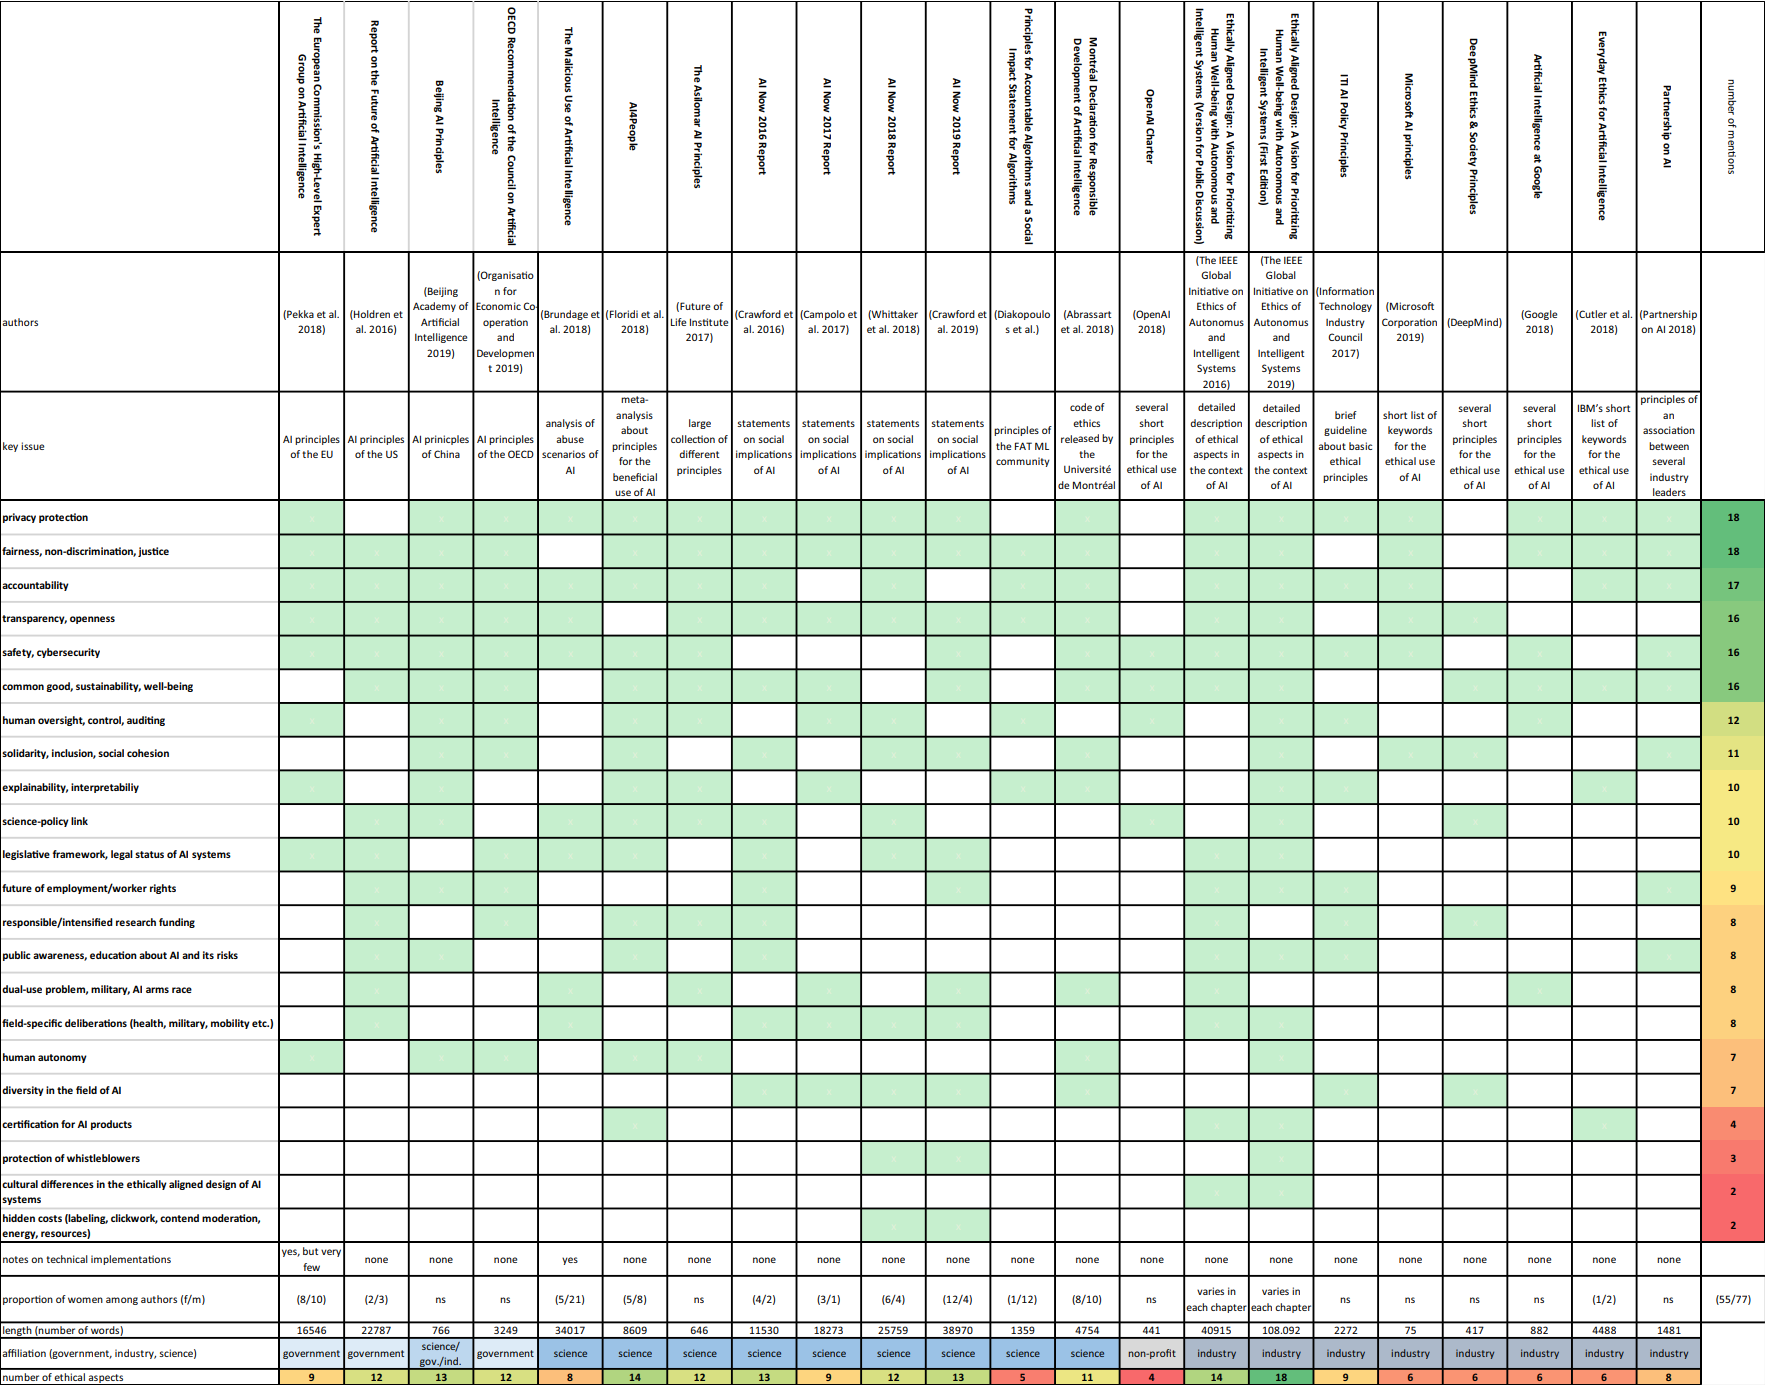
\includegraphics[width = \textwidth]{Bilder/Ethical huidelines hagendorf 2020.png}
            \caption{Übersicht ethischer Leitlinien und die Abgedeckten Aspekte \cite{Hagendorff2020}}
            \label{fig:EthikGuidelines}
        \end{figure} \\
        Um den aktuellen Stand der bereits existierenden Ethik Leitlinien wird die Abbildung \ref*{fig:EthikGuidelines} herangezogen.\cite{Hagendorff2020}

%#########################################
    \newpage
    \section{Vorurteile im Zusammenhang mit \ac{KI}}
    \label{subsec:KIundbias}
    \subsection{Bias}
    \label{subsubsec:Bias}
        - ML ist immer auf Basis von Daten aus der Vergangenheit 
        -   Begriffserklärung: Data Bias vs Bias Verzerrung\\
        -   Arten von Bias: \\
            -   Bias durch Abwesenheit - Wenn eine Info fehlt, kann das zu Diskriminierung führen. \\
            -   Diskriminierung durch Menschen. \\
        Arten von Bias: Cognitive, Social, Perceptual und Motivational Bias \cite{HEGKI2019Definition}\cite{Parkavi2018} \cite{Fabi2022}

    \subsection{Diskriminierung durch Vorurteile in Daten}
    \label{subsubsec:diskriminierungdurchverzerrung}

        - Wie funktioniert Bias in Daten
        - Was ist die Problematik
        - Welche Auswirkungen hat es 
        - Realbeispiele <-- Bewerbungsverfahren
        \cite{IncidentDatabase2015_16} \cite{hagendorff2019maschinelles}

    \subsection{Gegenma{\ss}nahmen}
    \label{subsubsec:gegenmassnahmen}
        - Was kann man dagegen tun?
        - Gibt es möglichkeiten Trainingsdaten künstlich zu erzeugen und so eine neutrale betrachtung zu schaffen
        - Parameter entfernen als Lösung --> Die KI wird aber dadurch schlechter 
        - 

        Wenn der Parameter mit dem Bias entfernt wird, wird das Ergebnis erstmal schlechter. 
        
    \newpage
\end{onehalfspace}